\chapter{Long-Lived Particles in ATLAS}

\label{ch:simulation}
% --------------------------------------------------------------------------------

As discussed in Section~\ref{sec:limitations}, various limitations in the \ac{SM} suggest a need for new particles at the \TeV scale. 
A wide range of extensions to the \acl{SM} predict that these new particles can have lifetimes greater than approximately one-hundredth of a nanosecond.
These include theories with universal extra-dimensions~\cite{extra_dim1, extra_dim2}, with new fermions~\cite{newfermions}, and with leptoquarks~\cite{leptoquark}.
As discussed in Section~\ref{sec:llp_theory}, many \ac{SUSY} theories also produce these \acp{LLP}, in both R-Parity violating~\cite{rpv1, rpv2, rpv3} and R-Parity conserving~\cite{rpc1, rpc2, rpc3, rpc4} formulations.
Split supersymmetry~\cite{split1, split2}, for example, predicts long-lived gluinos with O(\TeV) masses.
This search focuses specifically on the \ac{SUSY} case, but many of the results are generic to any model with \acp{LLP}. 

Long-lived gluinos or squarks carry color-charge and will thus hadronize into color neutral bound states called \rhadrons.
These are composit particles like the usual hadrons but with one supersymmetric constituent, for example $\tilde{g}q\bar{q}$ and $\tilde{q}\bar{q}$.
Through this hadronization process, the neutral gluino can acquire a charge.
Gluino pair production, $p p\rightarrow \tilde{g}\tilde{g}$ has the largest cross sectional increase with the increase in energy to 13 TeV, and so this search focuses on gluino \rhadrons.
Planned future updates will extend the case to explicitly include squark and chargino models, but the method covers any long-lived, charged, massive particle.

\section{Event Topology}
\label{sec:characteristics}

The majority of SUSY models predict that gluinos will be produced in pairs at the \ac{LHC}, through processes like $p p \rightarrow q\bar{q} \rightarrow \tilde{g}\tilde{g}$ and $p p \rightarrow g g \rightarrow \tilde{g}\tilde{g}$, where the gluon mode dominates for the collision energy and gluino masses considered for this search.
During their production, the long-lived gluinos hadronize into color singlet bound states including $\tilde{g}q\bar{q}$, $\tilde{g}qqq$, and even $\tilde{g}g$~\cite{rhadron}.
The probability to form the gluon-only bound states is a free parameter usually taken to be 0.1, while the meson states are favored among the \rhadrons~\cite{rhad_atlas}.
The charged and neutral states are approximately equally likely for mesons, so the \rhadrons will be charged roughly 50\% of the time.

These channels produce \rhadrons with large \pt, comparable to their mass, so that they typically propagate with $0.2 < \beta < 0.9$~\cite{rhad_atlas}.
The fragmentation that produces that hadrons is very hard, so the jet structure around the \rhadron is minimal, with less than 5 \GeV of summed particle momentum expected in a cone of $\Delta R < 0.25$ around the \rhadron~\cite{rhad_atlas}.
After hadronization, depending on the gluino lifetime, the \rhadrons then decay into hadrons and a \ac{LSP}~\cite{rhadron}.

In summary, the expected event for pair-produced long-lived gluinos is very simple: two isolated, high-momentum \rhadrons that propagate through the detector before decaying to jets.
The observable features of such events depend strongly on the interaction of the \rhadron with the material of the detector and also its lifetime.
Section~\ref{sec:rh_interactions} describes the interactions of \rhadrons which reach the various detector elements in ATLAS and Section~\ref{sec:rh_lifetimes} provides a summary of the observable event descriptions for \rhadrons of various lifetimes.

\subsection{Detector Interactions}
\label{sec:rh_interactions}

After approximately 0.2 ns, the \rhadron reaches the pixel detector. If charged, it deposits energy into the material through repeated single collisions that result in ionization of the silicon substrate~\cite{pdg}. 
Because of its comparatively low $\beta$, the ionization energy can be significantly greater than expected for \ac{SM} particles because the most-probable energy loss grows significantly as $\beta$ decreases~\cite{pdg}.
This large ionization can be measured through the \ac{ToT} read out from the pixel detector as described in Section~\ref{sec:pixel_dedx}.
Large ionization in the inner detector is one of the major characteristic features of \acp{LLP}.

Throughout the next few nanoseconds, the \rhadron propagates through the remainder of the inner detector.
A charged \rhadron will provide hits in each of these systems as would any other charged particle, and can be reconstructed as a track.
The track reconstruction provides a measurement of its trajectory and thus its momentum as described in Section~\ref{sec:tracks}.
The large momentum is another characteristic feature of massive particles produced at the \ac{LHC}.
\textbf{Note: At this point I am failing to mention that the TRT provides a possible dE/dx measurement, because no one uses it as far as I know.}

As of roughly 20 ns, the \rhadron enters the calorimeter where it interacts hadronically with the material.
Because of its large mass and momentum, the \rhadron does not typically stop in the calorimeter, but rather deposits a small fraction of its energy through repeated interactions with nucleons.
The probability of interaction between the gluino itself and a nucleon is low because the cross section drops off with the inverse square of its mass, so the interactions are primarily governed by the light constituents~\cite{g4_rhad_2009}.
Each of these interactions can potentially change that quark content and thus change the sign of the \rhadron, so that the charge at exit is typically uncorrelated with the charge at entry~\cite{rhad_atlas}.
The total energy deposited in the calorimeters during the propagation is small compared to the kinetic energy of the \rhadron, around 20-40 \GeV, so that \ep is typically less than 0.1~\cite{rhad_atlas}.

Then, 30 ns after the collision, it reaches the muon system, where it again ionizes in the material if charged and can be reconstructed as a muon track.
Because of the charge-flipping interactions in the calorimeter, this track may have the opposite sign of the track reconstructed in the inner detector, or there may be a track present when there was none in the inner detector and vice-versa.
The propagation time at the typically lower $\beta$ results in a significant delay compared to muons, and that delay can be assessed in terms of a time-of-flight measurement.
Because of the probability of charge-flip and late arrival, there is a significant chance that an \rhadron which was produced with a charge will not be identified as a muon.
The long time-of-flight is another characteristic feature of \rhadrons which are reconstructed as muons.

\subsection{Lifetime Dependence}
\label{sec:rh_lifetimes}

The above description assumed a lifetime long enough for the \rhadron to exit the detector, which through this search is referred to as ``stable'', even though the particle may decay after exiting the detector.
There are several unique signatures at shorter lifetimes where the \rhadron decays in various parts of the inner detector; these lifetimes are referred to as ``metastable''.

The shortest case where the \rhadron is considered metastable is for lifetimes around 0.01 ns, where the particle decays before reaching any of the detector elements.
Although the \rhadrons are produced opposite each other in the transverse plane, each \rhadron decays to a jet and an \ac{LSP}.
The \acp{LSP} are not measured, so the produced jets can be significantly imbalanced in the transverse plane which results in large missing energy.
That missing energy can be used to trigger candidate events, and provides the most efficient trigger option for shorter lifetimes.
Additionally, the precision of the tracking system allows the displaced vertex of the \rhadron decay to be reconstructed from the charged particles in the jet.
The distance of that vertex from the interaction point can be used to distinguish \rhadron decays from other processes.
Figure~\ref{fig:rhadron_displaced} shows a schematic diagram of an example \rhadron event with such a lifetime.
The diagram is not to scale, but instead illustrates the detector interactions in the pixel detector, calorimeters, and muon system.
It includes a representation of the charged \rhadron and the neutral \rhadron, as well as the \acp{LSP} and jets (shown as charged hadrons) produced in the decay.
Neutral hadrons may also be produced in the decay but are not depicted.
Previous searches on ATLAS have used the displaced vertex to target \ac{LLP} decays~\cite{SUSY-2014-02}.

\begin{figure}[h!]
\centering
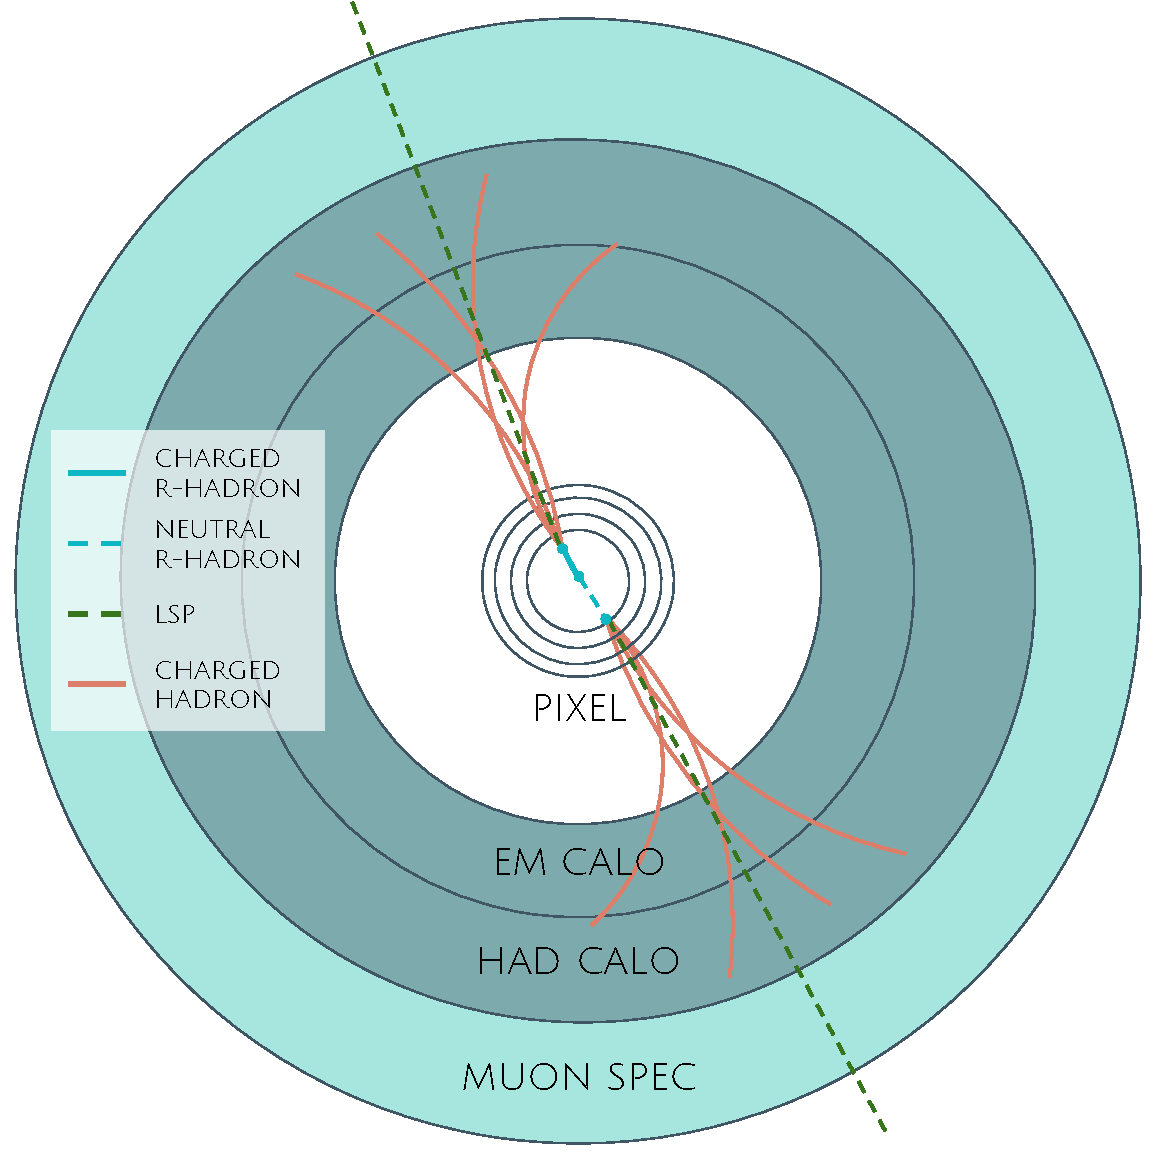
\includegraphics[width=\halffig]{figures/rhadron_displaced.pdf}
\caption{A schematic diagram of an \rhadron event with a lifetime around 0.01 ns. The diagram includes one charged \rhadron (solid blue), one neutral \rhadron (dashed blue), \acp{LSP} (dashed green) and charged hadrons (solid orange). The pixel detector, calorimeters, and muon system are illustrated but not to scale.}
\label{fig:rhadron_displaced}
\end{figure}

The next distinguishable case occurs at lifetimes greater than 0.1 ns, where the \rhadron forms a partial track in the inner detector.
If the decay products are sufficiently soft, they may not be reconstructed, and this forms a unique signature of a disappearing track.
An example of such an event is illustrated in Figure~\ref{fig:rhadron_disappear}, which shows the short track in the inner detector and the undetected soft charged hadron and \ac{LSP} that are produced.
A dedicated search on ATLAS used the disappearing track signature to search for \ac{LLP} in Run 1~\cite{SUSY-2013-01}.
z\textbf{Note: might not be worth mentioning the disapearing track here since it is actually a chargino search, the soft pion is pretty unique to charginos.}

\begin{figure}[h!]
\centering
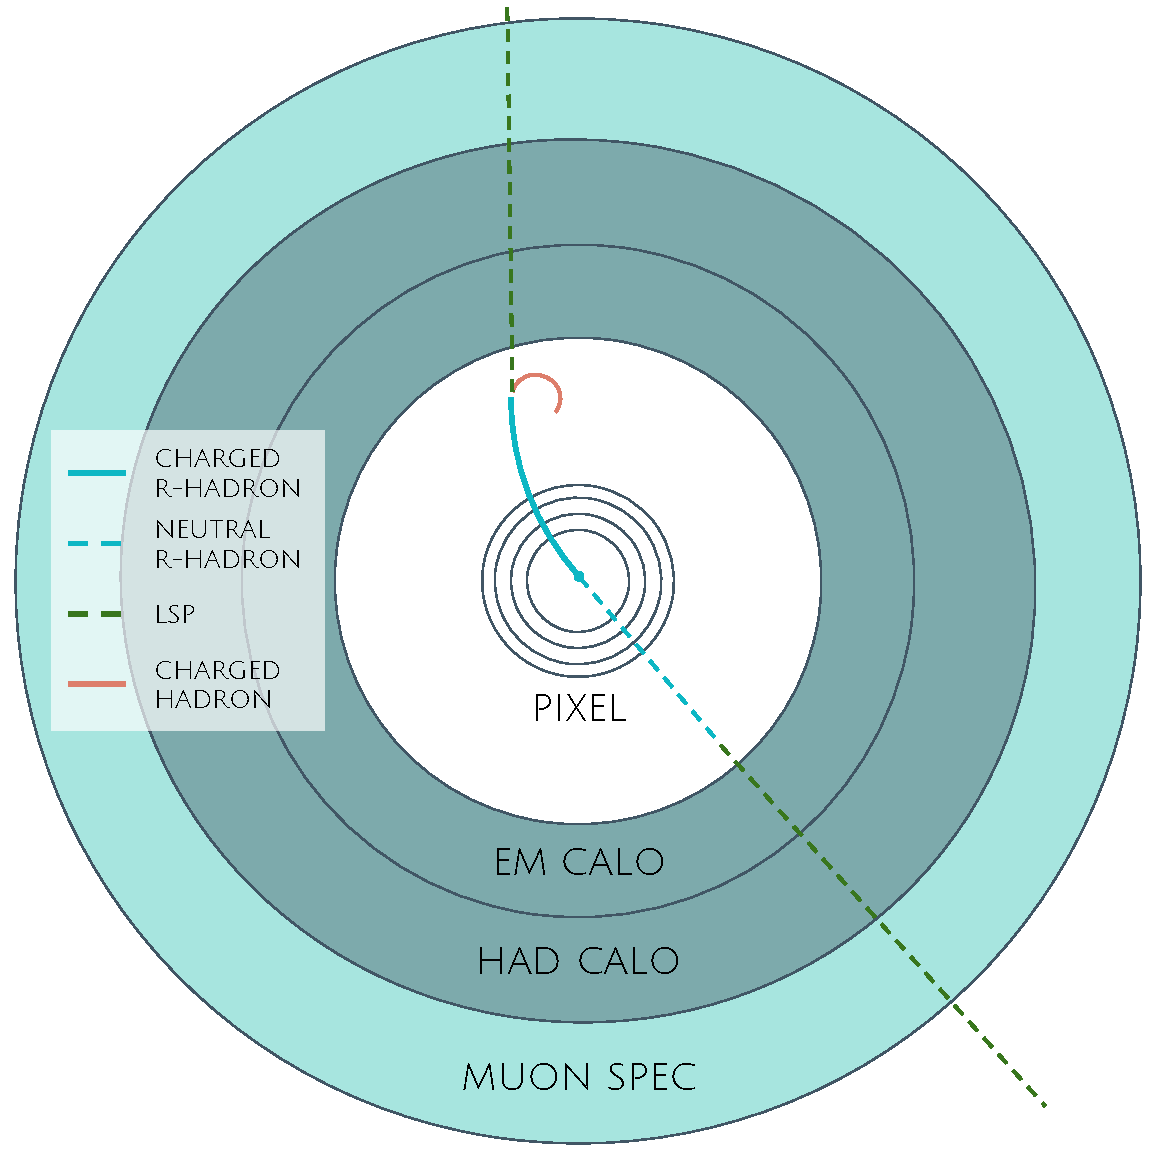
\includegraphics[width=\halffig]{figures/rhadron_disappear.pdf}
\caption{A schematic diagram of an \rhadron event with a lifetime around 4 ns. The diagram includes one charged \rhadron (solid blue), one neutral \rhadron (dashed blue), \acp{LSP} (dashed green) and a charged hadron (solid orange). The pixel detector, calorimeters, and muon system are illustrated but not to scale.}
\label{fig:rhadron_disappear}
\end{figure}

If the decay products are not soft, the \rhadron daughters form jets, resulting in an event-level signature of up to two high-momentum tracks, jets, and significant missing energy.
The missing energy has the same origin as in the case of 0.01 ns lifetimes, from the decay to unmeasured particles, and again can be large.
The high-momentum tracks will also have the characteristicly high-ioniziation of massive, long-lived paticles in the inner detector.
Figure~\ref{fig:rhadron_metastable_short} illustrates an example event with one charged \rhadron which decays after approximately 10 ns, and shows how the jets from the decay can still be reconstructed in the calorimeter.
Several previous searches on ATLAS from Run 1 have used this signature to search for \rhadrons~\cite{SUSY-2012-01, SUSY-2013-22}, including a dedicated search for metastable particles~\cite{SUSY-2014-09}.

\begin{figure}[h!]
\centering
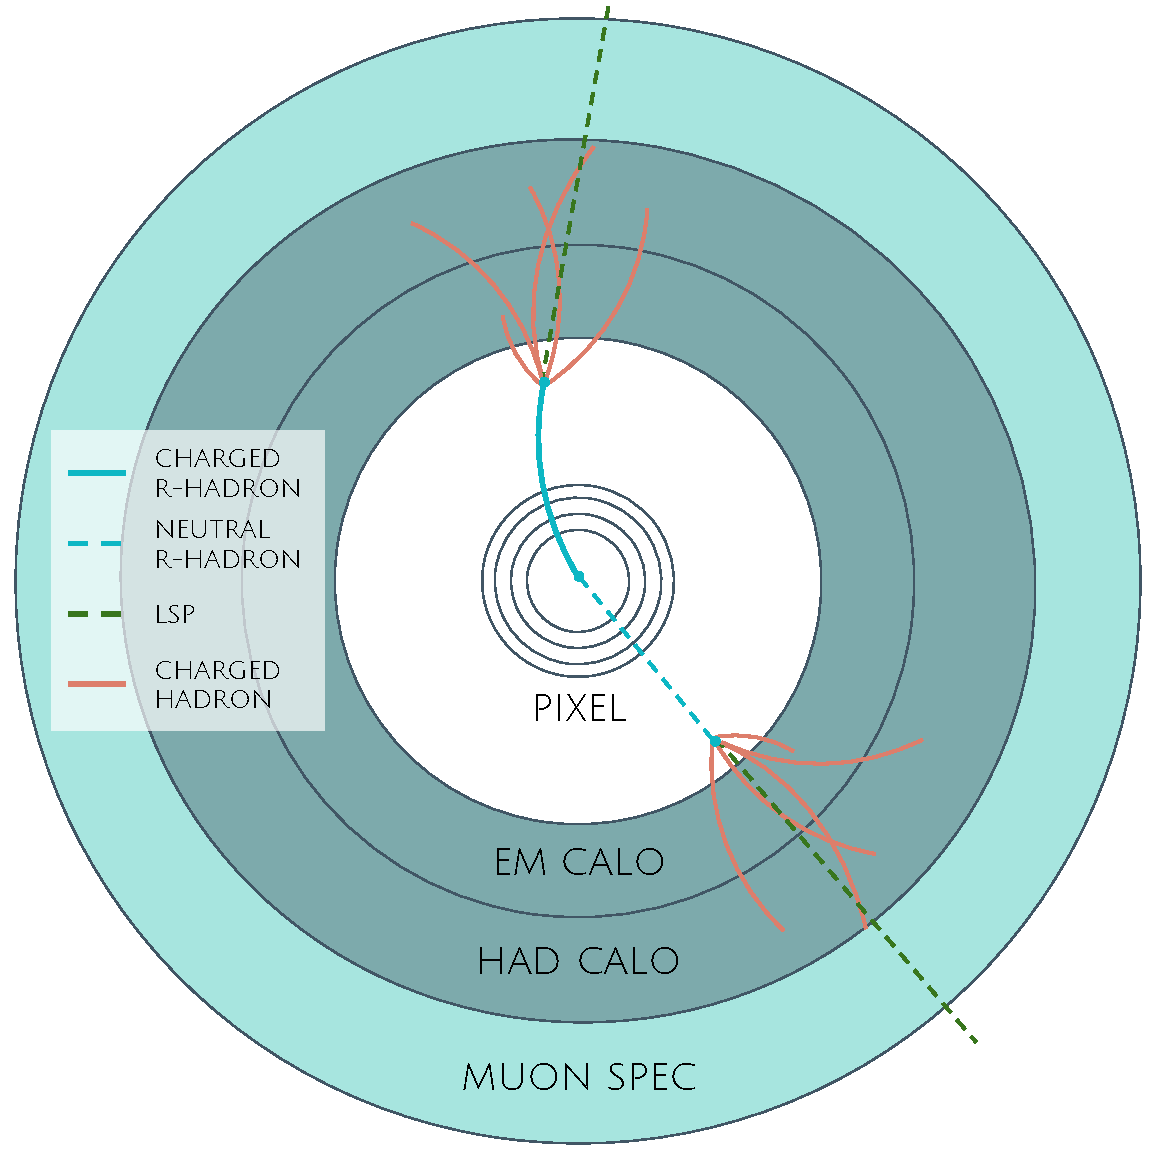
\includegraphics[width=\halffig]{figures/rhadron_metastable_short.pdf}
\caption{A schematic diagram of an \rhadron event with a lifetime around 5 ns. The diagram includes one charged \rhadron (solid blue), one neutral \rhadron (dashed blue), \acp{LSP} (dashed green) and charged hadrons (solid orange). The pixel detector, calorimeters, and muon system are illustrated but not to scale.}
\label{fig:rhadron_metastable_short}
\end{figure}


If the lifetime is longer than several nanoseconds, in the range of 15-30 ns, the \rhadron decay can occur in or after the calorimeters, but prior to reaching the muon system.
This case is similar to the above, although the jets may not be reconstructed, and is covered by many of the same search strategies.
The events still often have large missing energy, although it is generated through different mechanisms.
The \rhadrons do not deposit much energy in the calorimeters, so a neutral \rhadron will not enter into the missing energy calculation.
A charged \rhadron opposite a neutral \rhadron will thus generate significant missing energy, and close to 50\% of pair-produced \rhadron events fall into this category.
If both \rhadrons are neutral then the missing energy will be low because neither is detected.
Two charged \rhadrons will also result in low missing energy because both are reconstructed as tracks and will balance each other in the transverse plane.
A small fraction of the time, one of the charged \rhadron tracks may fail quality requirements and thus be excluded from the missing energy calculation and again result in signficant missing energy.
Figure~\ref{fig:rhadron_metastable_long} illustrates another example event with one charged \rhadron which decays after approximately 20 ns, and shows how the jets from the decay might not be reconstructed.

\begin{figure}[h!]
\centering
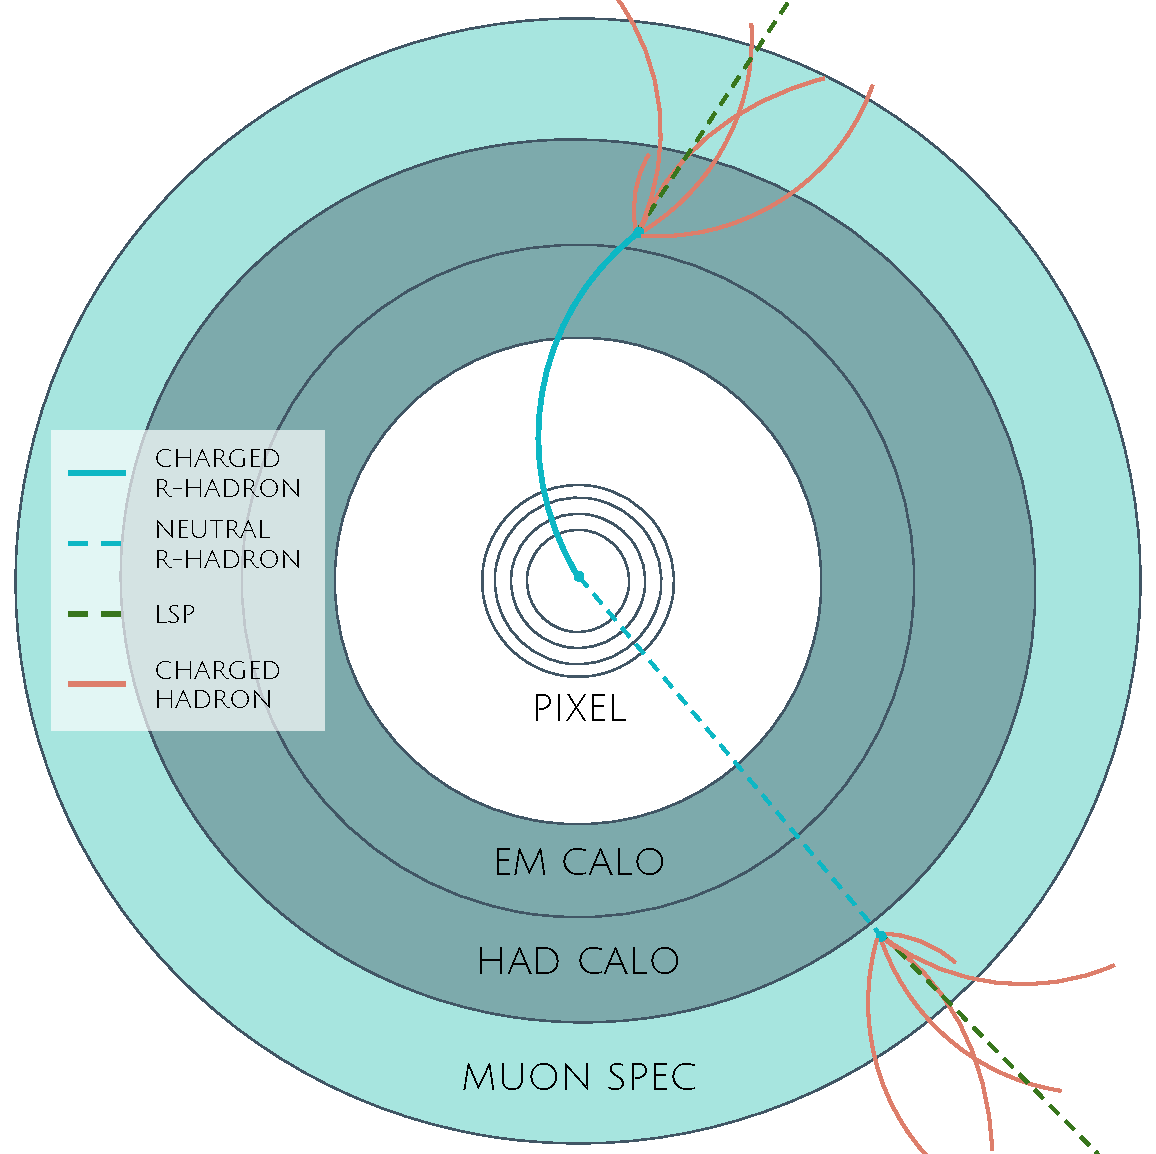
\includegraphics[width=\halffig]{figures/rhadron_metastable_long.pdf}
\caption{A schematic diagram of an \rhadron event with a lifetime around 20 ns. The diagram includes one charged \rhadron (solid blue), one neutral \rhadron (dashed blue), \acp{LSP} (dashed green) and charged hadrons (solid orange). The pixel detector, calorimeters, and muon system are illustrated but not to scale.}
\label{fig:rhadron_metastable_long}
\end{figure}


The longest lifetimes, the stable case, has all of the features of the 30-50 ns case but with the addition of muon tracks for any \rhadrons that exit the calorimeter with a charge.
That muon track can provide additional information from time-of-flight measurements to help identify \acp{LLP}.
An example of the event topology for one charged and one neutral stable \rhadron is shown in Figure~\ref{fig:rhadron_stable}.
Some searches on ATLAS have included this information to improve the search reach for stable particles~\cite{SUSY-2013-22, stable2016}.

\begin{figure}[h!]
\centering
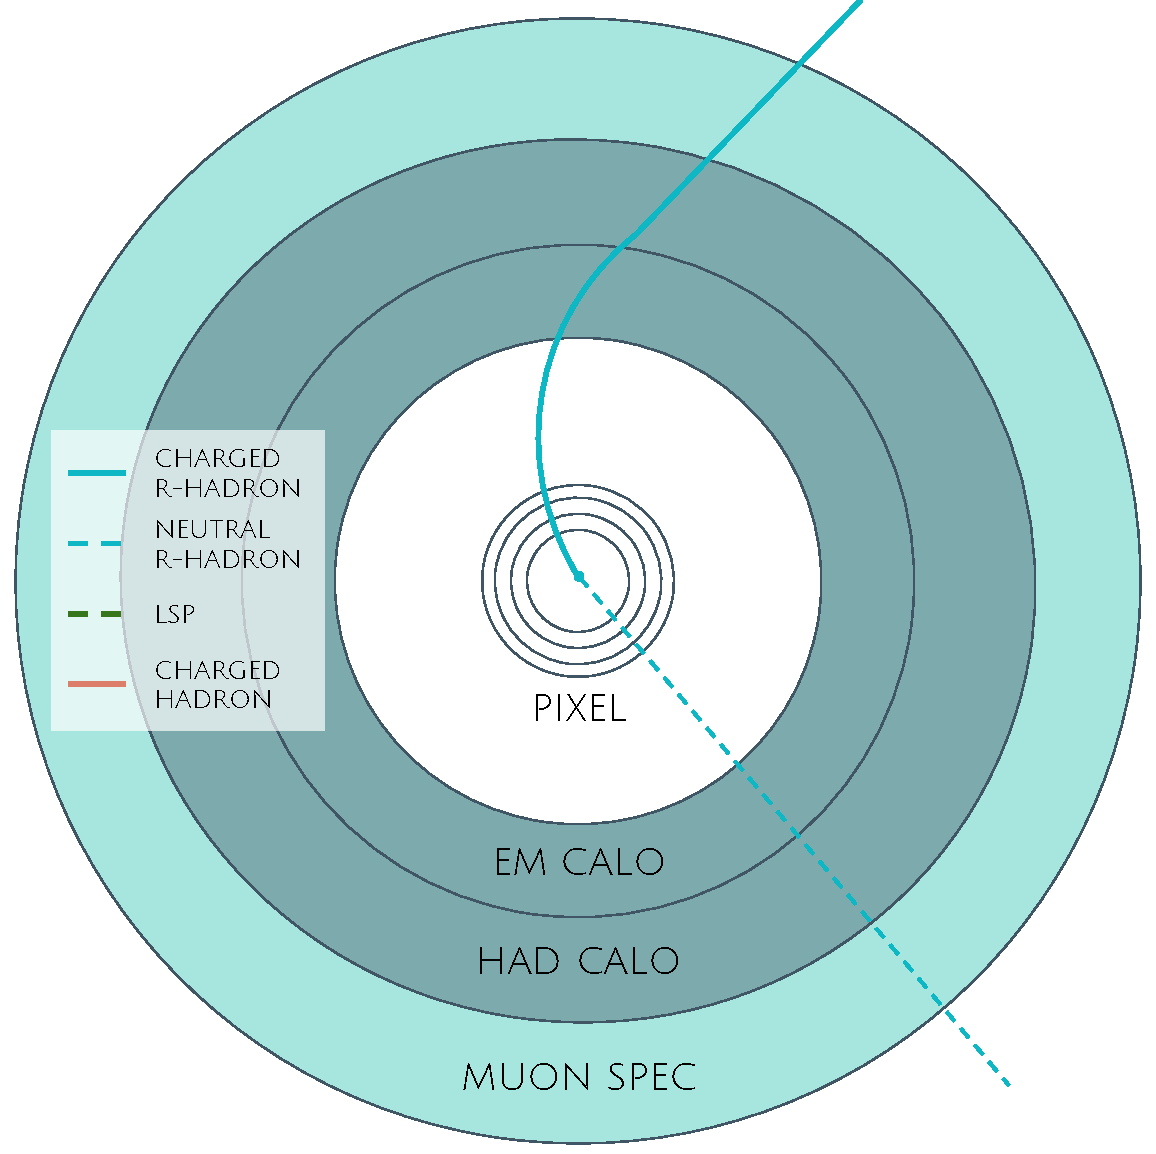
\includegraphics[width=\halffig]{figures/rhadron_stable.pdf}
\caption{A schematic diagram of an \rhadron event with a lifetime around 20 ns. The diagram includes one charged \rhadron (solid blue) and one neutral \rhadron (dashed blue). The pixel detector, calorimeters, and muon system are illustrated but not to scale.}
\label{fig:rhadron_stable}
\end{figure}


% ----------------------------------------

\section{Simulation}
% Discuss the details of mass/lifetime points for the R-Hadrons
\label{sec:simulation_samples}

All of the event topologies discussed above are explored by simulations of \rhadron events in the ATLAS detector. 
A large number of such samples are generated to determine signal efficiencies, to measure expected yields, and to estimate uncertainties. 
The primary interaction, pair production of gluinos with masses between 400 and 3000 \GeV, is simulated using \texttt{Pythia 6.4.27}~\cite{pythia6}  with the AUET2B~\cite{ATL-PHYS-PUB-2011-014} set of tuned parameters for the underlying event and the CTEQ6L1~\cite{CTEQ} \ac{PDF} set.
The simulated interactions include a modeling of pileup by adding secondary, minimum bias interactions from both the same (in-time pileup) and nearby (out-of-time pileup) bunch crossings.
This event generation is then augmented with a dedicated hadronization routine to hadronize the long-lived gluinos into final states with \rhadrons~\cite{heavy_hadronization}, with the probability to form a gluon-gluino bound set at 10\%~\cite{Fairbairn:2006gg}.

The cross sections used for these processes are calculated at \ac{NLO} in the strong coupling constant with a resummation of soft-gluon emmision at \ac{NLL}~\cite{Beenakker:1996ch,Kulesza:2008jb,Kulesza:2009kq,Beenakker:2009ha,Beenakker:2011fu}.
The nominal predictions and the uncertainties for each mass point are taken from an envelope of cross-section predictions using different \ac{PDF} sets and factorization and renormalization scales~\cite{Kramer:2012bx}.

The \rhadrons then undergo a full detector simulation~\cite{}, where the interactions of the \rhadrons with the material of the detector are described by dedicated \texttt{Geant4}~\cite{GEANT4} routines. 
These routines model the interactions described in Section~\ref{sec:rh_interactions}, including the ionizing interactions in the silicon modules of the inner detector and the \rhadron-nucleon interactions in the calorimeters~\cite{Mackeprang:2006gx, Mackeprang:2009ad}.
The specific routine chosen to describe the interactions of the \rhadrons with nucleons, the ``generic model'', uses a pragmatic approach where the scattering cross section is taken to be a constant 12 mb per light quark.
In this model the gluino itself does not interact at all except through its role as a reservoir of kinetic energy.

The lifetimes of these \rhadrons are then simulated at several working points, $\tau = 0.1, 1.0, 3.0, 10, 30, 50$ and detector stable, where the particle is required to decay after propagating for a time compatible with its lifetime.
Only one decay mode is simulated for these samples, $\tilde{g} \rightarrow q\bar{q}\tilde{\chi}_1^0$ with the neutralino mass set to 100 \GeV, which is chosen because it has the highest sensitivity among all of the modes studied in previous searches~\cite{SUSY-2014-09}.
Heavier neutralinos have similar results but generate less missing energy which reduces the efficiency of triggering.

All of the simulated events are then reconstructed using the same software used for collision data.
The fully reconstructed events are then reweighted to match the distribution of initial state radiation in an alternative sample of events, 
generated with \texttt{MG5\_aMC@NLO}~\cite{madgraph}, which has a more accurate description of radiate effects than \texttt{Pythia6}.
This reweighting provides a more accurate description of the momentum of the gluino-gluino system and is important in modeling the efficiency of triggering and offline event selection.


% ----------------------------------------
